\chapter{General framework of the project}
\section*{Introduction}
In this chapter we will present a global overview of the project, starting with the presentation of the host organization, followed by the problematic that was the reason behind the project, and finally we will into the methodology that was adopted to achieve this project objectives.
\section{The Host Organization}
\paragraph[short]{ADACTIM}
helps businesses leverage technology to improve their operations. They specialize in cloud computing, application integration and management, enterprise resource planning (ERP), and business intelligence (BI).  They operate internationally across Europe, North Africa, and Africa.

\begin{figure}[H]
    \centering
    \frame{
\includegraphics[width=0.5\columnwidth]{logo-adactim.png}}
    \caption{Logo Entreprise Adactim}
    \label{fig:logo_Adactim}
\end{figure}

\subsection*{ \textbullet\ Adactim  Mission}
ADACTIM can enable a company to benefit from technological transformations in the areas of IT infrastructure and integrated business systems allowing it to focus its energy on its core business.
\\
\emph{"Their mission is to facilitate businesses' access to technological innovations, to simplify their daily use, allowing the company to be more efficient and competitive.
With this, the client company can focus its resources on its development and its customers. the company will be well-equipped with business software and IT infrastructure and outsource appropriate operations processes."}\cite{adactim}
\section{Problematic}

\subsection{Existing study}
\noindent
\textbf{Description of the Current Environment:}
\\
Some applications that are managed by ADACTIM currently runs on a manually provisioned Azure cloud infrastructure managed through the web portal. Which means the actions to these infrastructures are done through a graphical interface provided by azure.
\\
\textbf{Analysis of Existing Deployment Processes:}

\begin{figure}[H]
    \centering
    \frame{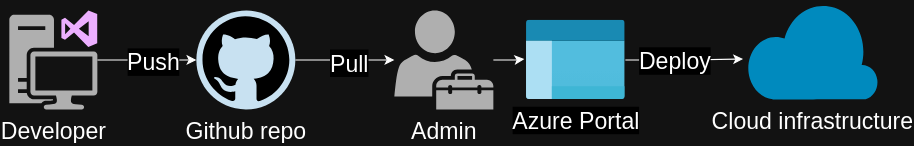
\includegraphics[width=0.8\columnwidth]{existing_stratigy.png}}
    \caption{existing strategy of the application deployment}
    \label{fig:existing_strategy}
\end{figure}

The deployment of applications in our current setup involves several steps, including code preparation, testing, deployment scheduling, and monitoring. Each deployment requires coordination between multiple teams, including developers, quality assurance, and system administrators.
Strengths and Weaknesses of the Current Approach:
\\
\textbf{Strengths:}
\begin{itemize}
    \item Our current deployment process follows a structured workflow, ensuring thorough testing before releasing applications into production.
    \item Effective communication and collaborative problem-solving are facilitated by teamwork during deployments.
\end{itemize}
\textbf{Weaknesses:}
\begin{itemize}
    \item Extended outages caused by inefficient deployment practices negatively impact business continuity and revenue.
    \item Limited automation in certain areas leads to manual errors and delays during deployments.
\end{itemize}
\noindent
\subsection{Problematic}
\par
While our current deployment process prioritizes rigorous testing and cross-team collaboration, it faces significant challenges impacting both efficiency and reliability. One critical issue lies in the protracted nature of deployment timelines. This stems from the inherent complexity of coordinating and executing numerous manual testing processes. Consequently, not only are the releases of crucial applications delayed but the potential for human error during manual interventions is also amplified
\par
In essence, our current application deployment process faces a critical challenge: balancing the strengths of its structured workflow and collaborative approach with the need for faster, more automated deployments.

\section{Proposed Deployment Optimization Solution}
In order to address the identified challenges, we propose a solution that leverages modern technologies and methodologies like Devops.
\begin{itemize}

    \item \textbf{Provisioning and Configuration Management:}
          Automate the provisioning and configuration of cloud infrastructure and application environments to ensure consistency and reliability using Infrastructure as Code (IaC) and Configuration Management tools.

    \item \textbf{Automating the build and testing process:}
          minimize manual intervention and expedite development cycles by leveraging automation across the build and testing pipeline. This not only reduces human error but also frees up valuable time for developers to focus on core tasks.
    \item \textbf{implementing a Deployment strategy:}
          Implement a deployment strategy that leverages automation to ensure seamless and efficient application deployments, minimizing downtime and errors. By applying these pattern principles:
          \begin{itemize}
              \item \textbf{Rightsize resources for each environment:} ensuring that the resources allocated to each environment are appropriate for the expected load. We can do this by implementing workspaces in Terraform.
              \item \textbf{Delete non-production environments:} ensuring that non-production environments are deleted when they are no longer needed.
          \end{itemize}
\end{itemize}

\section{Methodology of the project}
While some projects might seem straightforward, a defined methodology is crucial for achieving success. This framework provides a roadmap, ensuring tasks are completed efficiently and in the right order. By following a methodology, we can avoid common pitfalls, manage our time effectively, and ultimately deliver a successful project.
\subsection*{ \textbullet\ Agile vs traditional methodologies}
\begin{longtable}[c]{
    |p{.45\textwidth}
    |p{.45\textwidth}|
    }
    \caption{the significant differences between traditional and agile project methodologies. \cite{TradvsAgile1}}
    \label{tab:traditional_vs_agile}                                                           \\
    \hline
    \textbf{ Traditional Methodology }         & \textbf{ Agile Methodology }                  \\
    \hline
    The Waterfall model is used.               & Iterative and incremental development.        \\
    \hline
    Emphasis on planning and design.           & Emphasis on flexibility and adaptability.     \\
    \hline
    Emphasis on deliverables and completion    & Emphasis on customer satisfaction             \\
    \hline
    Projects are completed in phases.          & Projects are completed in sprints.            \\
    \hline
    The strict change management process.      & Encourages changes and improvements.          \\
    \hline
    Team roles and responsibilities are fixed. & Team roles and responsibilities are flexible. \\
    \hline
    Limited customer involvement               & High customer involvement                     \\
    \hline
    Risk management is proactive               & Risk management is reactive                   \\
    \hline
\end{longtable}
the choice between agile and traditional methodologies hinges on how much flexibility is needed. Agile thrives on an iterative approach. The team continuously works in short cycles, delivering features and gathering feedback to adapt and refine the project as it goes. This makes it ideal for DevOps, where requirements can evolve quickly. Traditional methods, on the other hand, emphasize upfront planning with a detailed roadmap. While this can be beneficial for projects with clear goals from the beginning, it can hinder DevOps teams who need to be adaptable and responsive to new information or feedback throughout the project lifecycle.
\subsection*{ \textbullet\ The Agile methodology}
\emph{"While seemingly designed for larger teams, Agile methodologies offer valuable structure even for single-person projects. Their core principles of iterative development, continuous improvement, and flexibility empower individuals to efficiently manage projects."}\cite{TradvsAgile}
\textbf{scrum:} Scrum is an agile framework that helps teams structure their work into short development cycles called sprints. Scrum teams commit to shipping work at the end of each sprint and adopt practices and a team structure that helps them achieve this cadence. Scrum takes the agile principles one step further, creating a structure that helps teams live the agile principles in their day-to-day work. Scrum is a well-documented agile framework that many teams can adopt without much disruption.
\subsection*{ \textbullet\ Verdict}
Considering the project's potential for evolving requirements and the benefits of iterative development, Scrum emerges as the optimal choice. Its focus on defined sprints, adaptability, and a structured approach to project management, even for solo developers, aligns perfectly with our project needs.

\begin{figure}[H]
    \centering
    \frame{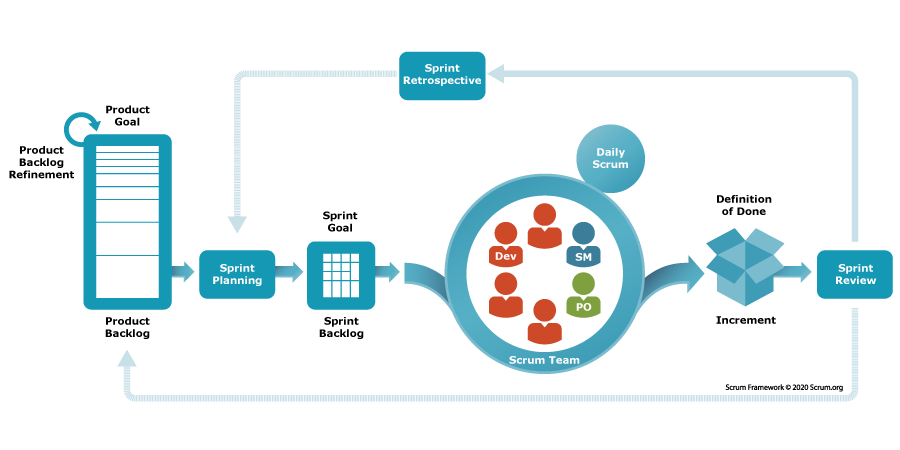
\includegraphics[width=0.8\columnwidth]{scrum-framework-9.29.23.png}}
    \caption{Scrum process \cite{TradvsAgile}}
    \label{fig:scrum_process}
\end{figure}

By following the Scrum process and maintaining open communication, we can ensure a successful project that delivers value iteratively while continuously adapting to feedback and changes.

\section*{Conclusion}
This chapter outlined the challenges associated with our current applications deployment process, which prioritizes thorough testing and collaboration but suffers from lengthy timelines and manual errors. To address these shortcomings, we proposed a new approach that leverages modern technologies and methodologies to achieve faster, more reliable deployments.
\par
The proposed solution emphasizes automation throughout the deployment lifecycle, encompassing infrastructure provisioning, build and testing processes, and the deployment strategy itself. This will minimize manual intervention, reduce errors, and expedite deployments. Additionally, the strategy incorporates security best practices and performance optimization techniques to ensure the applications' continued reliability and availability.
\par
Finally, we discussed the methodology Scrum that will be adopted to manage the project. This agile framework will provide a structured approach to project management.
\par
The next chapter, we will provide a comprehensive exposition to many concepts in the field of DevOps and cloud computing, which will be prove essential to understanding the project's technical aspects.